Adapt your algorithm and code from (a) to the eigenvalue boundary value problem

$$
u''(x) = \lambda u(x), \; u(0) = 0, u'(1) + u(1) = 0
$$

for which eigenvalues cannot be computed explicitly. Plot the first few eigenfunctions.

\begin{solution}\ \\\\
    \ \\
    \newpage
    \hfill\vfill

    \pagebreak
    
    \noindent The first four eigenvalues for this problem with various mesh sizes are listed below:

    \begin{figure}[h]
        \begin{verbatim}
              n       lambda_1  lambda_2   lambda_3  lambda_4
            5.0000    -4.0546   -23.4452   -58.4449   -99.1976
           50.0000    -4.1146   -24.1170   -63.5285  -122.4306
          100.0000    -4.1155   -24.1334   -63.6239  -122.7652
          200.0000    -4.1158   -24.1378   -63.6500  -122.8569
          300.0000    -4.1158   -24.1387   -63.6550  -122.8747
          400.0000    -4.1158   -24.1390   -63.6568  -122.8809
        \end{verbatim}
        \caption{Output of \texttt{problem\_1b.m}}
    \end{figure}

    We plot the first four eigenvectors corresponding to these eigenvalues below:


    \begin{figure}[h]
        \centering
        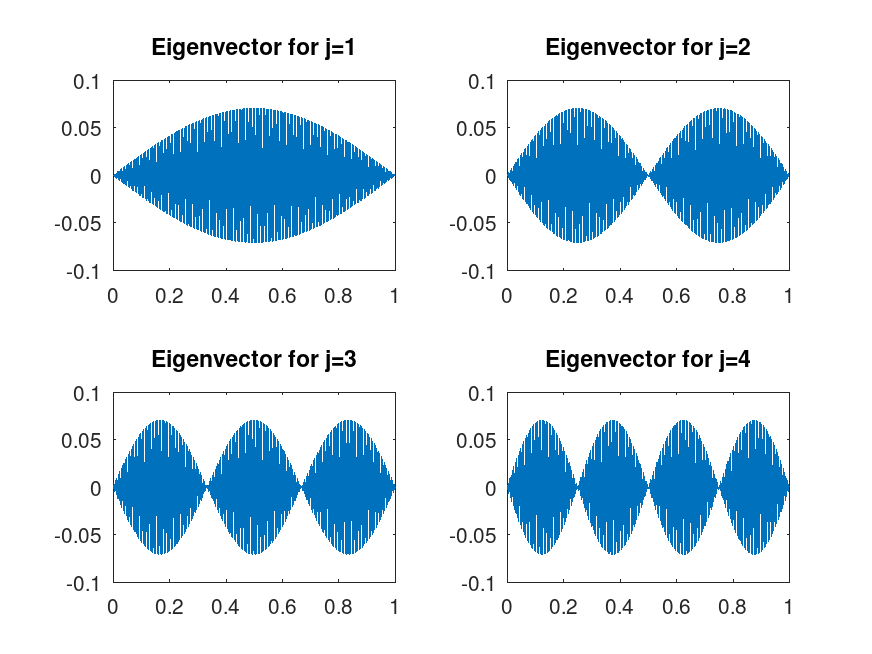
\includegraphics[width=0.85\textwidth]{problem_1b_eigenvectors.png}
        \caption{Eigenvectors for 1D eigenvalue mixed BVP}
    \end{figure}
\end{solution}